\documentclass[a4paper]{spie}  %>>> use for US letter paper
%\renewcommand{\baselinestretch}{1.3}   %>>> 1.65 for double spacing

\usepackage[]{graphicx}
\usepackage{hyperref}
\usepackage{listings}
\hypersetup{
    colorlinks,
    linkcolor={black!50!black},
    citecolor={blue!50!black},
    urlcolor={blue!80!black}
}
\usepackage{pdfpages}
\usepackage{parcolumns}

\usepackage[utf8]{inputenc} 
\usepackage[english]{babel}

\usepackage{color}
\definecolor{lightgray}{rgb}{.9,.9,.9}
\definecolor{darkgray}{rgb}{.4,.4,.4}
\definecolor{purple}{rgb}{0.65, 0.12, 0.82}


\usepackage{array}
\newcolumntype{L}[1]{>{\raggedright\let\newline\\\arraybackslash\hspace{0pt}}m{#1}}
\newcolumntype{C}[1]{>{\centering\let\newline\\\arraybackslash\hspace{0pt}}m{#1}}
\newcolumntype{R}[1]{>{\raggedleft\let\newline\\\arraybackslash\hspace{0pt}}m{#1}}

\usepackage{xcolor,colortbl}
\usepackage{color}
\usepackage{babelbib}


\title{Robot Applications} 

\author{Lars Engel, Vikash, Ahsan Yousuf
\\\textit{\\Faculty of Computer Science and Electrical Engineering
\\Fachhochschule Kiel: University of Applied Sciences\\ Sokratespl. 1, 24149 Kiel, Germany}
}


\setcounter{page}{1}
\pagestyle{plain} 

\date{\today}  
 
  \begin{document} 
  
  \begin{LARGE}
  \maketitle
  \end{LARGE}
  \vspace{60pt}
  \begin{large}
  \tableofcontents
  \newpage

%%%%%%%%%%%%%%%%%%%%%%%%%%%%%%%%%%%%%%%%%%%%%%%%%%%%%%%%%%%%% 


\section{Introduction}
Just a short introduction for motivation of project (why should we let the robot play this game?)
\clearpage
\section{Background}
\subsection{Explanation and Description of Robot}
\subsection{Explanation and Description of Camera}
\subsection{Explanation and Description of Ninemens Morris}
\subsection{Explanation and Description of the AI}
\subsection{Setup}
The setup of the project is shown in Figure \ref{setup_overview}. The robot is mounted on the table. It is connected via a LAN cable to a switch. The camera is attached to a beam at a fixed position and is also connected to the same switch. This way the robot and the camera will be in the same network and can communicate with each other.
\begin{figure}[h]
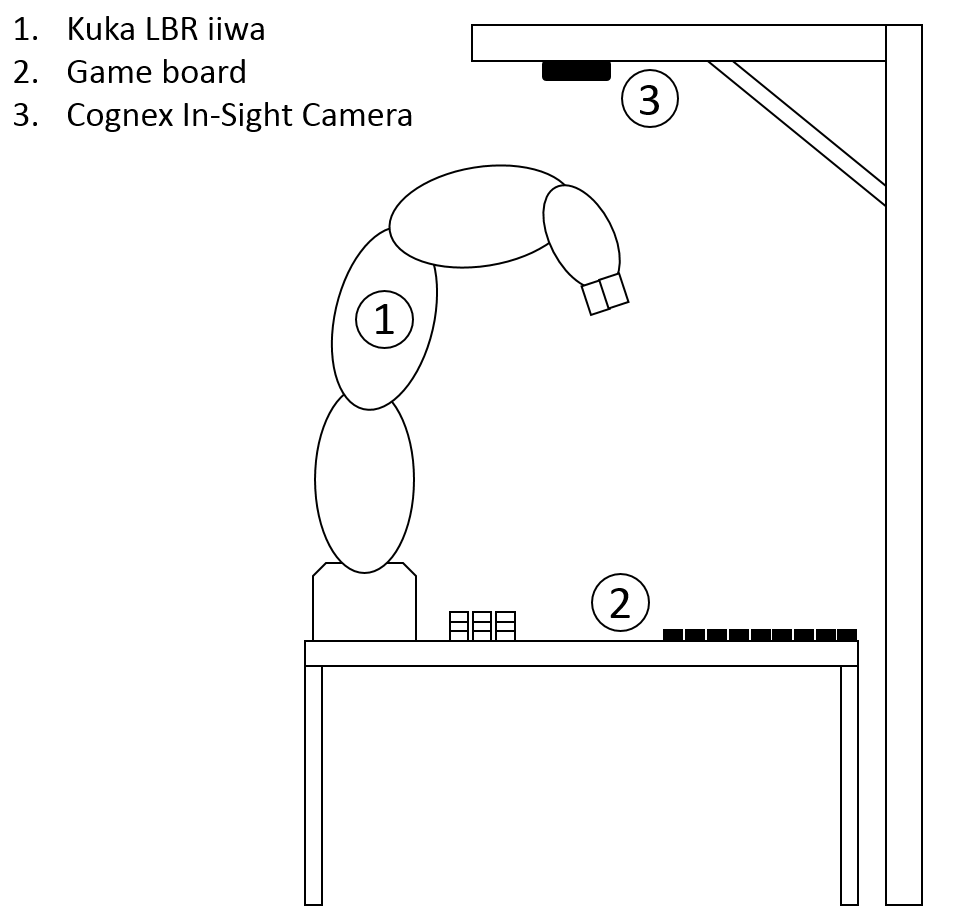
\includegraphics[width=13cm]{images/setup_overview.png}
\centering
\caption{A sketch of the setup of the project. (Not true to scale)}
\label{setup_overview}
\end{figure}
\clearpage
\section{Implementation}
\subsection{Work on the artificial intelligence}
To simplify the use of the AI, some code was written directly into the classes of the AI. The most important class of the AI, which is responsible for organizing the game flow, is the \emph{GameController}. It runs in an own thread and is started by the \emph{MainController}, which is also part of the AI. (See Figure \ref{thread_diagram})\\
To be able to use the self written classes inside of the GameController, it was necessary to forward the classes, that where instantiated inside the robot thread, through the MainController to the GameController.
\begin{figure}[h]
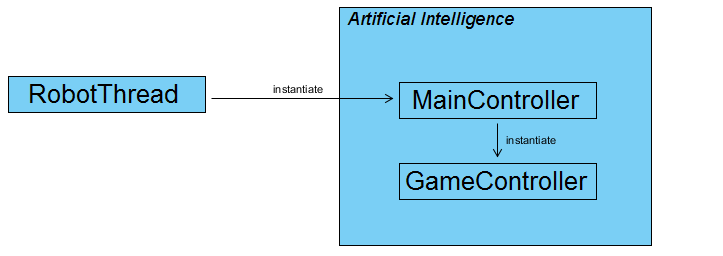
\includegraphics[width=15cm]{images/diagram.png}
\centering
\caption{The MainController thread is started by the robot thread. The MainController then starts the GameController thread.}
\label{thread_diagram}
\end{figure}
\subsection{Description of own written classes}
\subsubsection{RobotInteractions}
The \emph{RobotInteractions} class shown in Figure \ref{class_roboInt} provides methods so that the robot can interact with the game. It contains for example the \emph{close()} and \emph{open()} methods to open and close the gripper of the robot. The method \emph{movePiece(AbstractFame origin, AbstractFrame destination)} can be used to move a game token from one position to another. It uses methods of the RobotMovements class to perform its movements.
\begin{figure}[h]
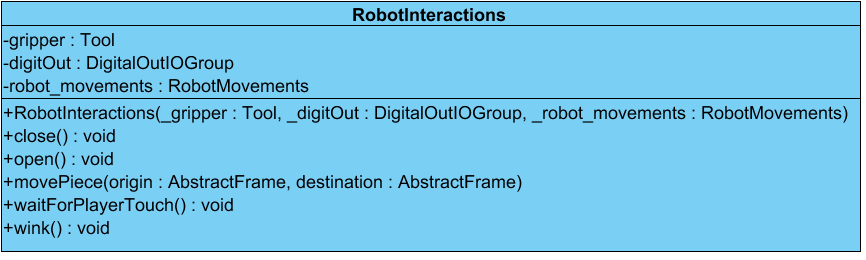
\includegraphics[width=15cm]{images/class_roboInt.png}
\centering
\caption{Class diagram of the RobotInteractions class}
\label{class_roboInt}
\end{figure}

\subsubsection{RobotMovements}
\begin{figure}[h]
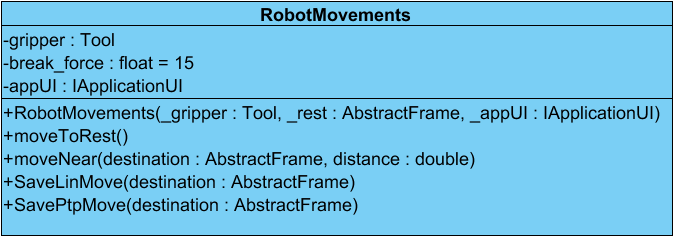
\includegraphics[width=12cm]{images/class_roboMov.png}
\centering
\caption{Class diagram of the RobotMovements class}
\label{class_roboMov}
\end{figure}
The RobotsMovements class shown in Figure \ref{class_roboMov} provides special movement methods like the \emph{moveToRest()} method which moves the robot to its rest position. It is important to move the robot to this position so that the camera, which is attached upright to the game board, can get a clear view (See Figure \ref{setup_overview}). \\
The class also provides the methods \emph{saveLinMove(AbstractFrame destination)} and \emph{savePtpMove(AbstractFrame destination)}. These are methods which where  created to enable safety for the human player. Since the robot is interacting in the same space where the human is also interacting, it is important to ensure that the human player will not be harmed by the robot. \\
\begin{figure}[h]
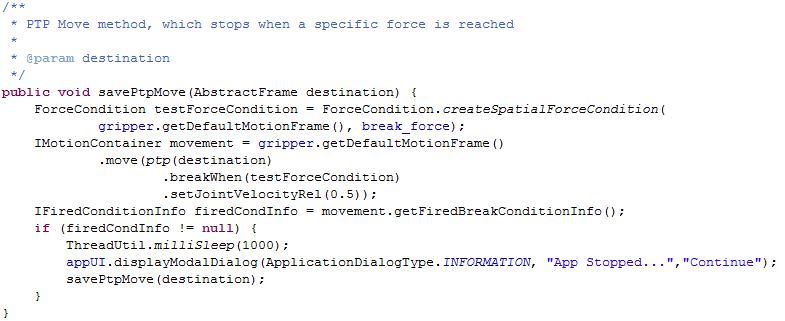
\includegraphics[width=18cm]{images/code_safety.png}
\centering
\caption{Code Listing of the RobotMovements class showing the SavePtpMove() method}
\label{code_safety}
\end{figure}
As shown in Figure \ref{code_safety} the \emph{savePtpMove(AbstractFrame destination)} method calls the \emph{move()} method of the \emph{IMotionContainer} class from the KUKA libraries with a \textit{breakWhen()} condition attached to that. This means that the movement will stop, when the specified ForceCondition will be fired. In case the ForceCondition was fired the movement will be stopped, the robot will wait for a second and a dialog will be shown on the KUKA Smartpad. The user then has to click on this dialog so that the movement can be repeated.
\subsubsection{Bordpoints}
\label{sec:boardpoints}
\begin{figure}[h]
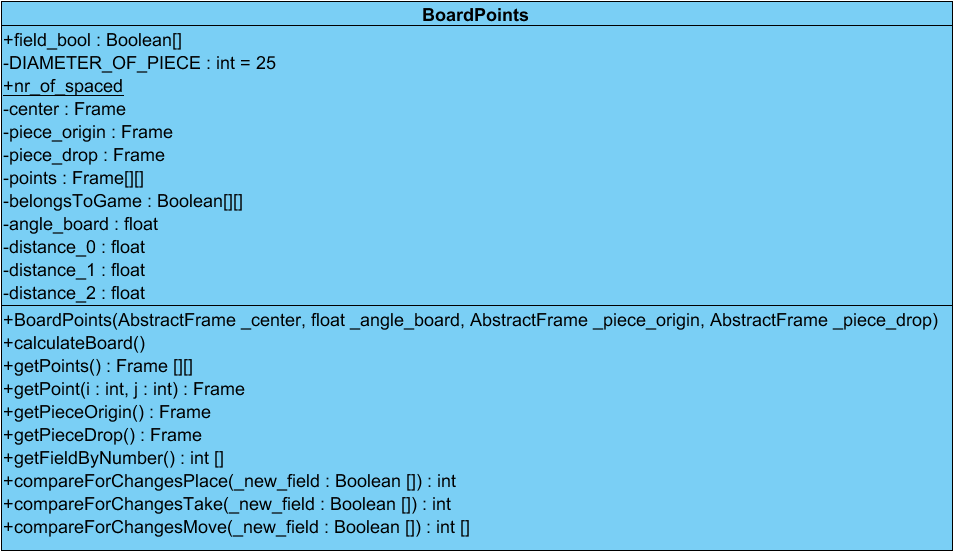
\includegraphics[width=15cm]{images/class_boPo.png}
\centering
\caption{Class diagram of the BoardPoints class}
\label{class_boPo}
\end{figure}
The BoardPoints class shown in Figure \ref{class_boPo} provides  all the information about important coordinates. At the start of the application this class calculates the coordinates for all 24 board points and stores them in a multidimensional array. \\
\begin{figure}[h]
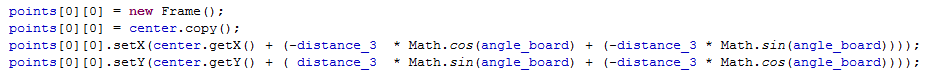
\includegraphics[width=17cm]{images/code_points_calc.png}
\centering
\caption{Code Listing of the Boardpoints class showing the board points calculation}
\label{code_points_calc}
\end{figure}
Figure \ref{code_points_calc} shows the calculation for the board point 0, 0 which is the point in the lower left corner. The calculation uses the center point of the board and the angle of rotation of the board to calculate the coordinates for each game point. The plan was to  get the center point and the angle of the board from the camera, but unfortunately the detection of the created jobs was not precise enough to get the correct angle of the board. So in this project the board needed to stay at a fixed angle. But with a correct working method to get the current angle from e.g. the camera this class is already prepared to compute the points based on the rotation of the board.

\subsubsection{Logger}
\begin{figure}[h]
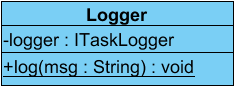
\includegraphics[width=4cm]{images/class_lo.png}
\centering
\caption{Class diagram of the Logger class}
\label{class_lo}
\end{figure}
The logger class shown in Figure \ref{class_lo} is instantiated as a static object in the main thread. This way logging information for debug messages or game messages could be used anywhere in the code.
\subsubsection{ModbusClient}
\begin{figure}[h]
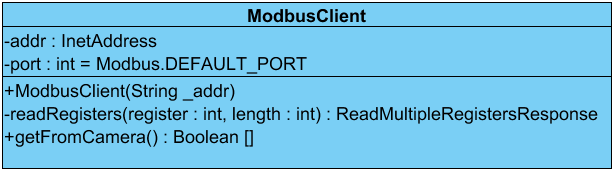
\includegraphics[width=12cm]{images/class_moCli.png}
\centering
\caption{Class diagram of the ModbusClient class}
\label{class_moCli}
\end{figure}
The ModbusClient class shown in Figure \ref{class_moCli} is responsible for the communication between the camera and the robot. As described in section \ref{commu} the communication is realized with Modbus/TCP. The ModbusClient class is instantiated inside the GameController of the artificial intelligence. The GameController calls the \emph{getFromCamera()} method which uses the \emph{readRegisters(int register, int length)} method to read the specified registers from the Modbus/TCP server provided by the camera. 

\subsection{Game Board}
The 24 points on the game board, where a game token can be placed are stored in two different formats:
\paragraph{6x6 Matrix of Game Points}
The artificial intelligence stores the game points in a multidimensional array with a size of six by six. Each array element is of type \emph{Token}, which is an enumeration, that can have either the value \emph{BLACK}, \emph{WHITE} or \emph{EMPTY}. The array serves as a 6x6 matrix. This matrix is visualized on the game board as shown in Figure \ref{setup_board}. It can be seen that not all fields of the matrix belong to the game. The points \{1,0\}, \{1,2\}, \{1,4\} and \{1,6\} for example do not belong to the game. Therefore the AI implements a method to compute all \emph{illegal game points}.\\
\begin{figure}[h]
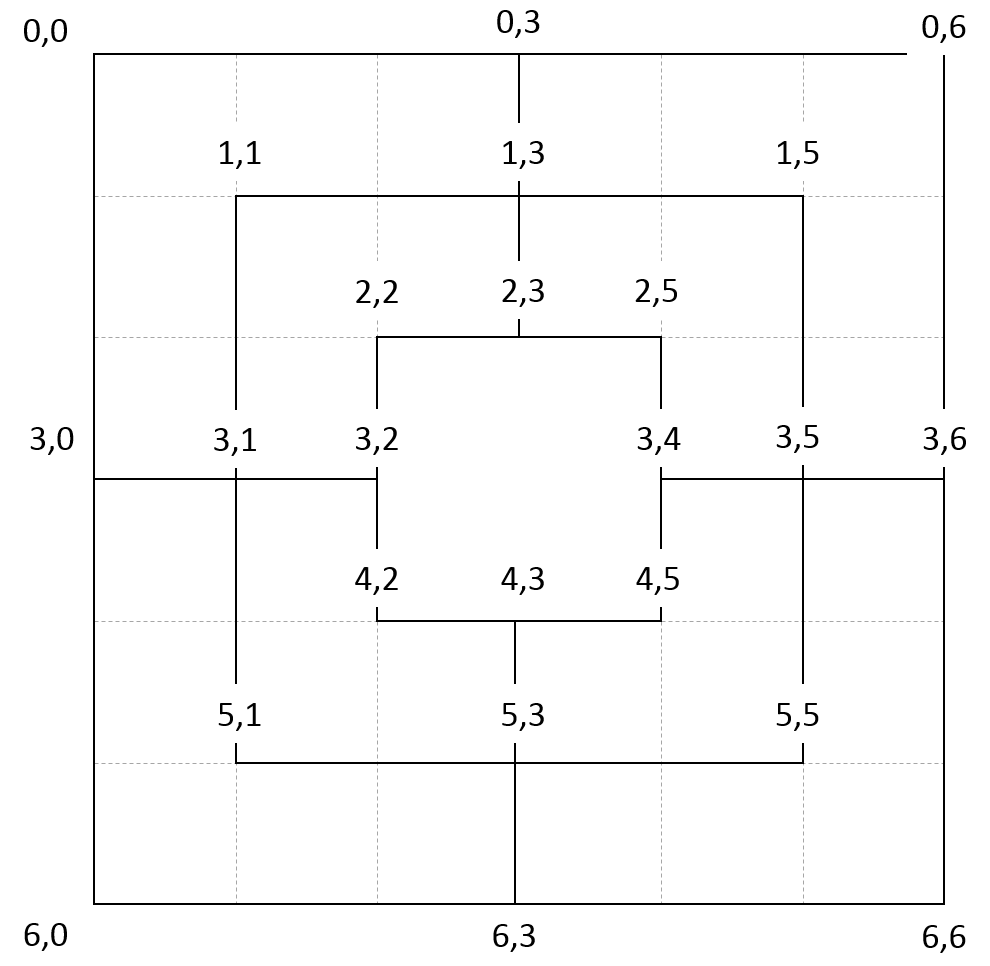
\includegraphics[width=10cm]{images/setup_board.png}
\centering
\caption{Setup of the Gameboard as a 6x6 matrix}
\label{setup_board}
\end{figure}
The coordinates for all game points are also stored as a multidimensional array with a size of six by six. This simplified the use of different methods provided by the AI, because no conversion between different formats was needed. For example the method \emph{getDest} of the class \emph{Move} from the AI returns the x and y coordinates of destination of the next move. These coordinates can be given to the \emph{RobotInteractions} class without conversion.
\paragraph{Array of 24 Boolean Values}
Information about the game board is also stored as an array of 24 boolean values. A field, where a game token is placed, has the value \emph{true} in this array. A field where no token is placed has the value \emph{false}. This format does not distinguish between black or white tokens. But since this information is stored in the AI, it is not necessary to store it again. The array is used for evaluating changes on the game board detected by the camera.

\subsection{Visual analysis}
\label{visual_analysis}
The visual analysis of the game was realized with a Cognex In-Sight 7000 Integrated Vision System. 
\subsubsection{In-Sight Explorer}
With the help of the Cognex In-Sight Explorer it was possible to create jobs to analyze the image captured by the camera.\\
\begin{figure}[h]
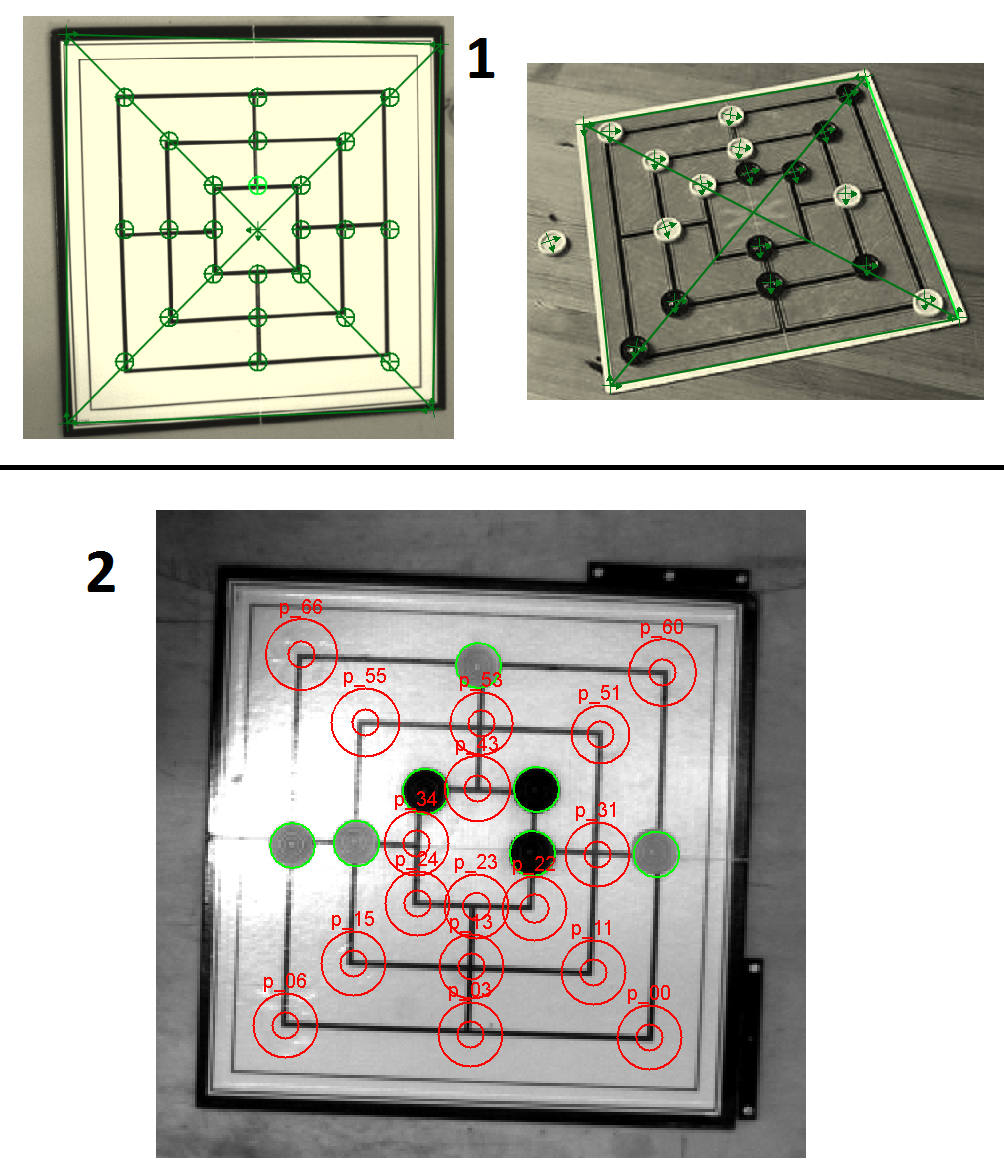
\includegraphics[width=15cm]{images/camera_00.png}
\centering
\caption{Different approaches for visual analysis}
\label{camera_00}
\end{figure}
It was the intention to create a job that can analyze the positions of game tokens on the board considering the rotation of the board. To accomplish this, the job should detect the corners of the game board. These corners then could be connected. The intersection between the two lines, that cross the game board will be the center of the game board (See Figure \ref{camera_00} part one). Comparing the angle of one of the lines with a reference line with an angle of 0 degrees provides the information about the rotation of the game board.\\ Unfortunately the detection of the board corners did not work as precise as needed. This lead to the problem that the rotation of the board could not be analyzed correctly. A wrong angle of the board would lead to wrong calculations for the board points. Since it is important, that the location of the board points are precise, so that the robot moves and takes pieces from the correct coordinates, the decision was made to use a fixed rotation for the game board. This is a limitation that could be resolved in a following project.\\
The detection of the tokens is realized with a tool of the In-Sight Explorer that detects circles at specific locations (See Figure \ref{camera_00} part two). It will output a message "available", if a circle was found at this location and another message "not available", if no circle was found at this location. The tool is not able to determine the color of the found circles. But since nine men's  morris is a game, that is played in turns, we can get the information about the color of the tokens within the robot application. On the downside, this limits the ability of cheat or misplaced game token detection.


\subsubsection{Communication between Robot and Camera}
\label{commu}
The communication as shown in Figure \ref{communication} uses the Modbus/TCP protocol. The camera acts as a Modbus/TCP server and the robot as Modbus/TCP client. The \emph{ModbusClient} class of the robot application (see Figure \ref{class_moCli})  sends a \emph{ReadMultipleRegistersRequest()} to the IP and port of the camera. The camera then sends the output of the visual analysis as TCP packages back to the robot application. The response of the camera is stored as an array of 24 boolean values inside the robot application where \emph{true} means a token was found and \emph{false} means no token was found at this location. This array can now be compared to the previously stored array \emph{field\_bool} in the \emph{BoardPoints} class (see Figure \ref{class_boPo}).
\begin{figure}[h]
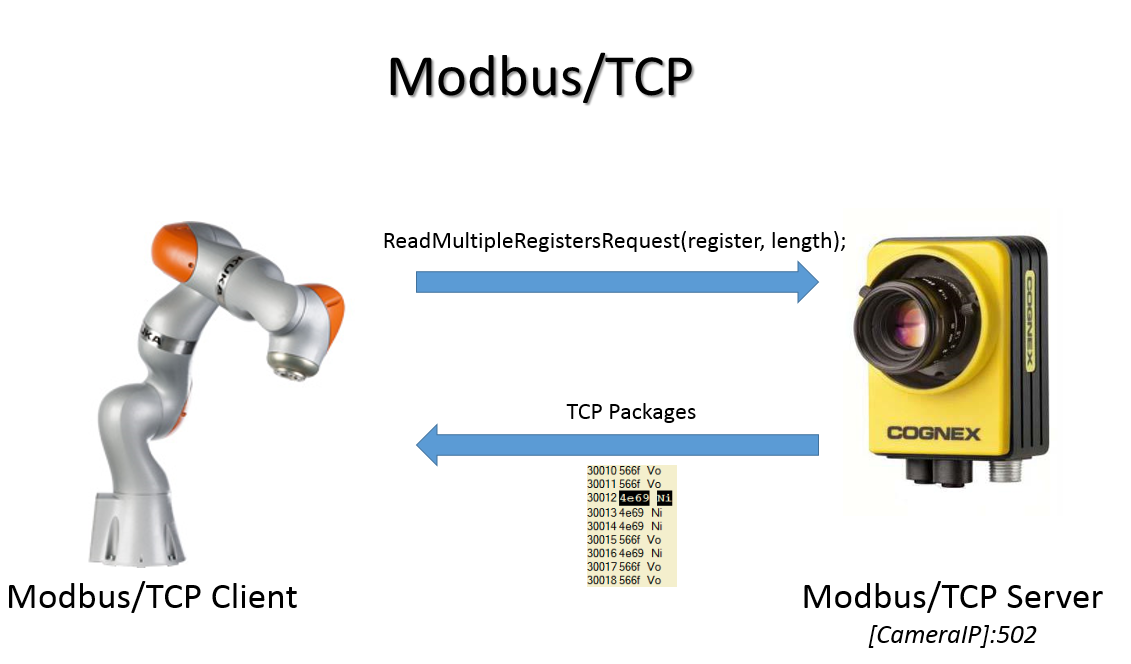
\includegraphics[width=15cm]{images/communication.png}
\centering
\caption{Communication between Camera and Robot}
\label{communication}
\end{figure}

\clearpage
\section{Conclusion and Future work}
The project was successfully completed since it is possible that a human can play Nine Men's Morris against the robot. The robot can sense and process its environment through the camera, so playing the game as a human feels very natural. The robot interacts with the human. He signalizes the human when it is his turn. \\ 
Though the final product is playable, there is still plenty of room for improvements:
\paragraph{Better cheat handling:} The cheat handling is very rudimentary right now. The AI detects when an illegal move is done and does not accept such a move. The robot will \emph{shake} when an illegal move is done. Unfortunately the human player now has to put back the tokens where they where before he cheated. If he does not remember where the token belongs the game can not be continued. An improvement would be to have the robot solve such a situation by placing a misplaced token where it belongs.
\paragraph{Board rotation:} As already mentioned in section \ref{visual_analysis} the game board has to be placed at a fixed angle. This limitation should be resolved in a future version of the application. The robot application is already prepared for such an improvement (see section \ref{sec:boardpoints}). A job for the camera, that is able to detect the rotation of the board precisely is necessary to resolve this situation. The best implementation would be a job that is not only able to detect the rotation of the board at the beginning of the game but also detect changes of the rotation and position of the game board while the game is running.   
\paragraph{Visual analysis:} The detection of the placed tokens is not very robust right now. It depends very much on the lightning how well the tokens can be recognized. Especially the white tokens are difficult to detect since, under sum conditions. Their contrast and color does not differ very much from the game board, which has a similar color since the camera is only detecting black and white. The camera that was available has only low features for visual analysis and the computational power is also low. Changing on a more powerful camera could make the application more robust. Since the robot application is not deeply connected to the visual analysis done by the camera, it would be very easy to exchange the camera. If the new camera could also be used as an Modbus/TCP server, no changes at all would be needed inside the robot application. 
\paragraph{Improvement of safety:} The implemented safety features could also be improved. The application will stop a movement if a specific \emph{ForceCondition} was fired. After that the robot will try to do the same movement again. But when a movement is not possible, because an immovable object is in its ways, this will lead to a infinite loop since the robot will try again and again to complete its movement. A better solution would be to enable the human player to stop the application, when the \emph{ForceCondition} was fired.
\paragraph{Human Computer Interaction:} To improve the usability and game play feeling the interaction between the human and the robot should be enhanced. It could be for example possible to implement speech recognition, so that the human player can say \emph{I am ready} to let the robot know, when it is his turn. The robot on the other hand could also say something to the human player to inform him about the game situation (e.g. \emph{Oh I have a mill, now I can take on of your tokens!}) or he could comment on movements of the human (e.g. congratulate for a good move).
\newpage

%%%%%%%%%%%%%%%%%%%%%%%%%%%%%%%%%%%%%%%%%%%%%%%%%%%%%%%%%%%%%
%%%%% References %%%%%
%\bibliographystyle{babunsrt-lf}
%\bibliographystyle{spiebib}   %>>>> makes bibtex use spiebib.bst
%\bibliography{references}   %>>>> bibliography data in report.bib

\end{large}
\end{document} 
